\documentclass[12pt,a4paper]{beamer}
\usepackage[utf8]{inputenc}
\usepackage{amsmath}
\usepackage{amsfonts}
\usepackage{amssymb, multicol}
\usepackage{framed}

\usepackage{graphicx}
\usepackage{caption}
\usepackage{subcaption}

\begin{document}
\begin{frame}

\[\textbf{Introduction to Statistics}\]
\end{frame}
\begin{frame}{Source}
\centering
Material, examples and data sets come from:\vspace{0.3cm}

\textbf{Open Intro Statistics, Second edition}\\
by\\
D.M.Diez, C.D.Barr and M. Cetinkaya-Rundel



\[\text{https://www.openintro.org/}\]
\end{frame}
\begin{frame}{Motivation}

\textbf{Case Study:}

\[\textbf{Q:}\text{ Does the use of stents reduce the risk of stroke?}\]
\end{frame}
\begin{frame}{Motivation}
\small\begin{itemize}
\item[]\textbf{Treatment group}. Patients in the treatment group received a stent and medical management. The medical management included medications, management of risk factors, and help in lifestyle modification.
\item[]\textbf{Control group}. Patients in the control group received the same medical management as the treatment group, but they did not receive stents.
\end{itemize}
\end{frame}
\begin{frame}{Motivation}
\textbf{Results from the stent study}
\begin{table}[h]
\centering
\resizebox{0.7\textwidth}{!}{
\begin{tabular}{l ccc}
\hline
Patient	&	group	&	0-30 days 	&	0-365 days \\
\hline
1		&	treatment &	no event &	no event \\
2		&	treatment &	stroke & stroke \\
3		&	treatment &	no event & no event \\
$\vdots$	&	$\vdots$	  &	$\vdots$ \\
450	&	control &	no event &	no event \\
451	&	control &	no event &	no event \\
\hline
\end{tabular}}
\end{table}
\end{frame}
\begin{frame}{Motivation}
\textbf{Summary of the stent study}
\begin{table}[h]
\centering
\resizebox{0.7\textwidth}{!}{
\begin{tabular}{l cc c cc}
& \multicolumn{2}{c}{0-30 days} &\hspace{5mm}\ & \multicolumn{2}{c}{0-365 days} \\
  \cline{2-3} \cline{5-6}
	& 	stroke 	& no event && 	stroke 	& no event \\
  \hline
treatment 	& 33		& 191	&&	45 	& 179 \\
control 		& 13		& 214	&& 	28	& 199 \\
  \hline
Total				& 46		& 405	&&	73	& 378 \\
  \hline
\end{tabular}}

\end{table}
\small\begin{itemize}
\setlength{\itemsep}{0mm}
\item Proportion who had a stroke in the treatment (stent) group: $45/224 = 0.20 = 20\%$.
\item Proportion who had a stroke in the control group: $28/227 = 0.12 = 12\%$.
\end{itemize}
\end{frame}
\begin{frame}{Motivation}
\begin{itemize}
\item An additional 8\% of patients in the treatment group had a stroke
\item This is contrary to what doctors expected, i.e. the stents would reduce the rate of strokes.
\item Statistical question: do the data show a "real" difference between the groups?
\end{itemize}

\end{frame}
\begin{frame}{Basics}
\begin{center}
\textbf{Statistics} is the study of how best to collect, analyse and draw conclusions from data.
\end{center}
\end{frame}
\begin{frame}{Basics}
\begin{itemize}
\item \textbf{Process of investigation}
\begin{itemize}
\item Identify a question or problem
\item Collect relevant data on the topic
\item Analyse the data
\item Form a conclusion
\end{itemize}
\end{itemize}
\end{frame}

\begin{frame}{Examples}
\textbf{Data Matrix} 
\begin{table}[t]
\centering
\resizebox{0.9\textwidth}{!}{
\begin{tabular}{cc ccc c}
  \hline
 & spam & num\_ char & line\_ breaks& format & number \\ 
  \hline
1 & no & 21,705 & 551 & html & small \\ 
  2 & no & 7,011 & 183 & html & big \\ 
  3 & yes & 631 & 28 & text & none \\ 
$\vdots$ & $\vdots$ & $\vdots$ & $\vdots$ & $\vdots$ & $\vdots$ \\
  50 & no & 15,829 & 242 & html & small \\ 
   \hline
\end{tabular}}
%\caption{Data matrix of \data{email50}. }
\end{table}
\end{frame}

% library(openintro); library(xtable); data(email50); email50[c(1,2,3,50),c("spam", "num_char", "line_breaks", "format", "number")]; xtable(email50[c(1,2,3,50),c("spam", "num_char", "line_breaks", "format", "number")], digits=0)

\begin{frame}{Variable description}
\begin{table}[t]
\center
\resizebox{0.9\textwidth}{!}{
\begin{tabular}{lp{10cm}}
\hline
{\bf variable} & {\bf description} \\
\hline
\bf spam & Specifies whether the message was spam \\
\bf num\_\hspace{0.3mm}char & The number of characters in the email   \\
\bf line\_\hspace{0.3mm}breaks & The number of line breaks in the email (not including text wrapping)   \\
\bf format & Indicates if the email contained special formatting, such as bolding, tables, or links, which would indicate the message is in HTML format    \\
\bf number & Indicates whether the email contained no number, a small number (under 1 million), or a large number   \\
\hline
\end{tabular}}
%\caption{Variables and their descriptions for the \data{email50} data set.\vspaceB{-3.5mm}}
\label{email50Variables}
\end{table}
\end{frame}

\begin{frame}{Types of Variables}
\begin{figure}
\centering
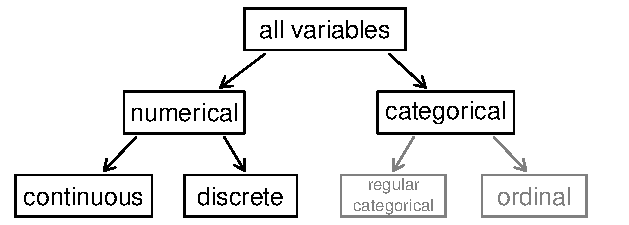
\includegraphics[width=1\textwidth]{variables}
%\caption{Breakdown of variables into their respective types.}
\label{variables}
\end{figure}
\begin{itemize}
\item[] \textbf{Numerical variables:} num\_ char, line\_ breaks
\item[]\textbf{Categorical variables:} spam, format, number
\end{itemize}
\end{frame}
\begin{frame}{Exploring numerical data}
	\begin{enumerate}
	\item  Scatterplots for paired data
	\item Dot plots and mean
	\item Histograms and Shape
	\item Variance and Standard deviation
	\item Box plots, quartiles and median
	\item Outliers and robust statistics
	\end{enumerate}
\end{frame}
\begin{frame}{Scatterplots}
	
	A \textbf{scatterplot} provides a case-by-case view of data for two numerical variables.
	\begin{figure}
	   \centering
	   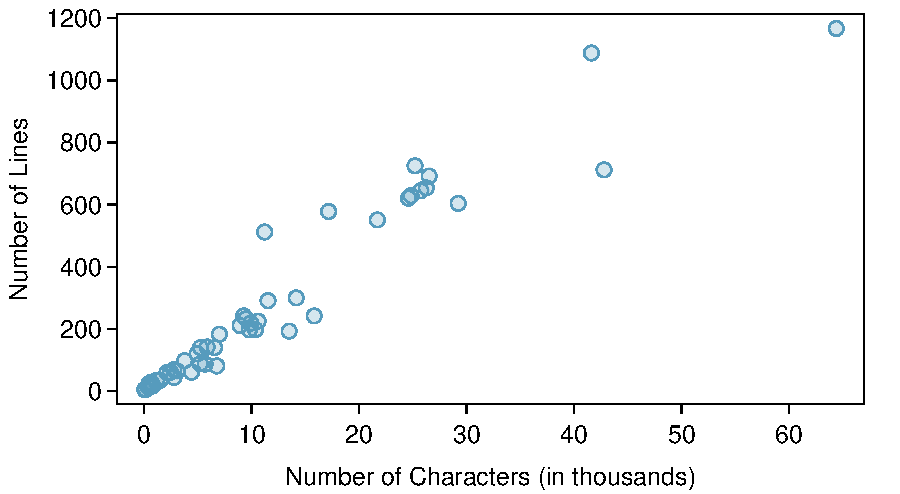
\includegraphics[width=0.75\textwidth]{email50LinesCharacters}
	   %\caption{A scatterplot of line\_\hspace{0.3mm}breaks versus num\_\hspace{0.3mm}char for the email50 data.}
	   \label{email50LinesCharacters}
	\end{figure}
	
\small Scatterplots are helpful in quickly spotting associations relating variables, whether those associations come in the form of simple trends or whether those relationships are more complex
\end{frame}
\begin{frame}{Scatterplots-Association}
	\begin{figure}
	   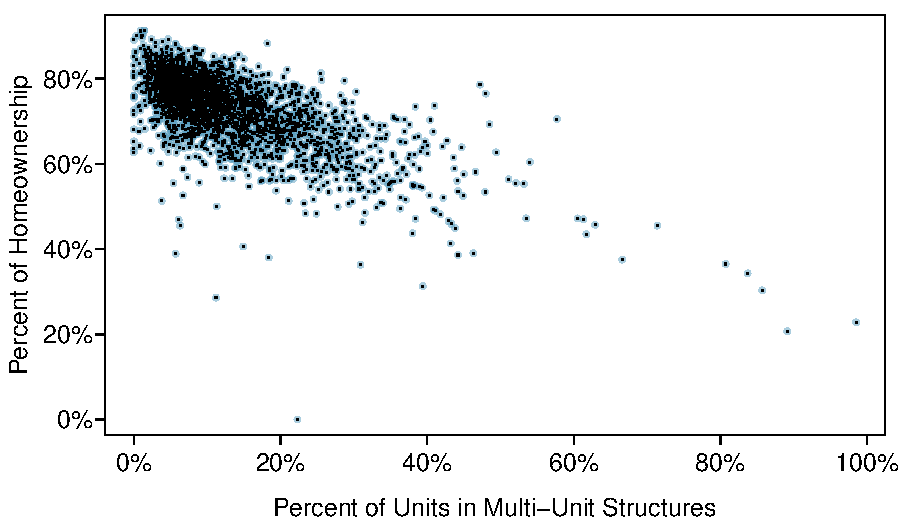
\includegraphics[width=0.5\textwidth]{figures/multiunitsVsOwnership/multiunitsVsOwnership}
	   \caption{Negative association}
	   \label{multiunitsVsOwnership}
	\end{figure}
	\begin{figure}
	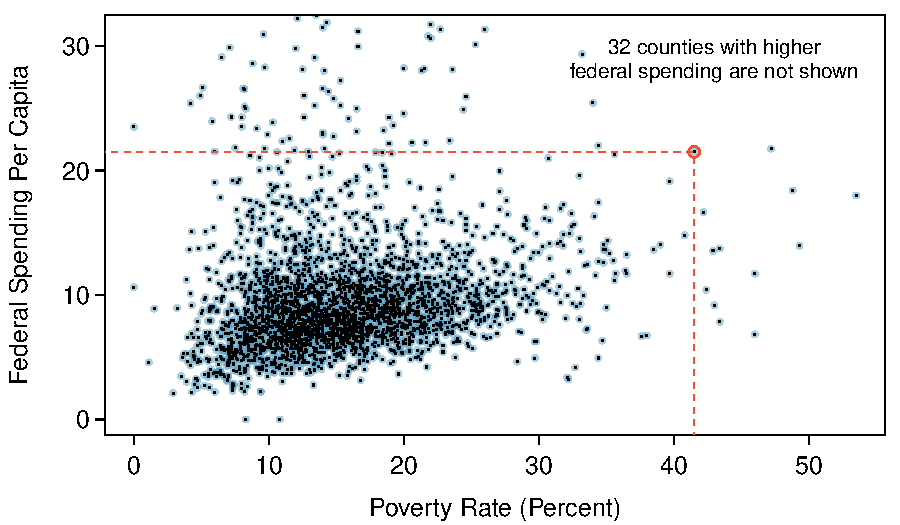
\includegraphics[width=0.5\textwidth]{figures/county_fed_spendVsPoverty/county_fed_spendVsPoverty}
	\caption{Positive association}
	\label{county_fed_spendVsPoverty}
	\end{figure}
\end{frame}
\begin{frame}{Scatterplots-Trends}
\begin{figure}
	\centering
		
	   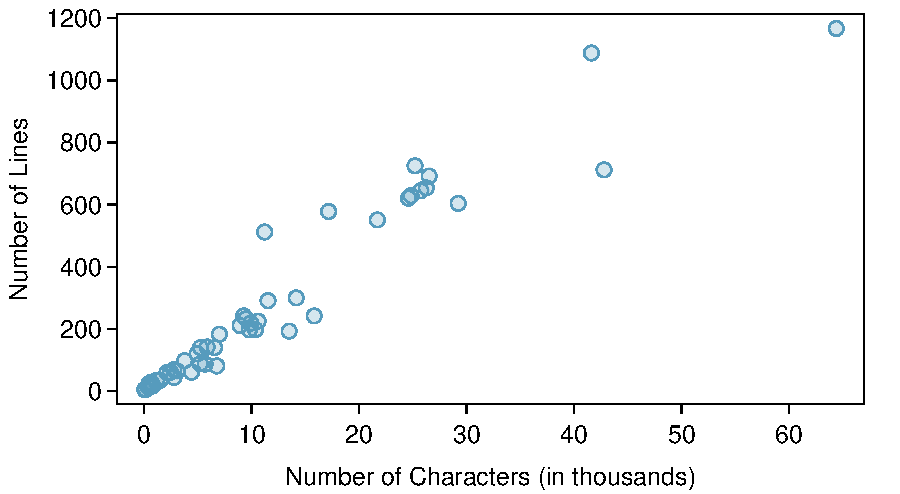
\includegraphics[width=0.5\textwidth]{email50LinesCharacters}
	   %\caption{A scatterplot of line\_\hspace{0.3mm}breaks versus num\_\hspace{0.3mm}char for the email50 data.}
\caption{Linear trend}
	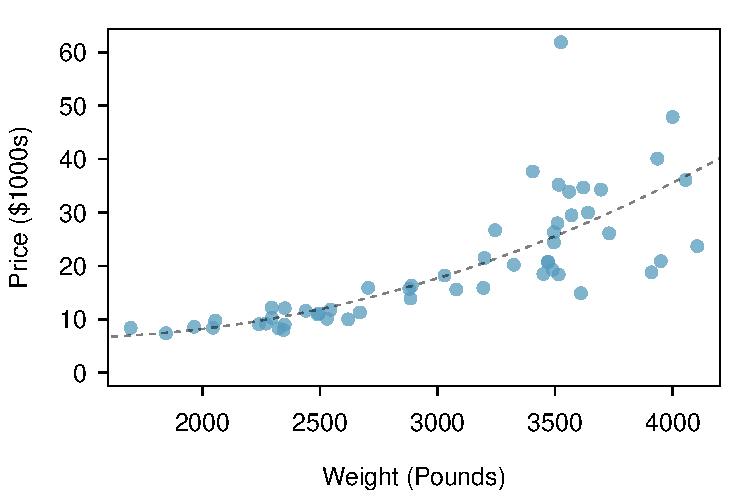
\includegraphics[width=0.5\textwidth]{figures/carsPriceVsWeight/carsPriceVsWeight}
	   %\caption{A scatterplot of price versus weight for 54 cars.}
\caption{Non-Linear trend}
	\end{figure}	
	%\small Because there is a downward trend in Figure~\ref{multiunitsVsOwnership} -- counties with more units in multi-unit structures are associated with lower homeownership -- these variables are said to be \textbf{negatively associated}{negative association}. A \textbf{positive association} is shown in the relationship between the poverty and fed\_\hspace{0.3mm}spend variables represented in Figure, where counties with higher poverty rates tend to receive more federal spending per capita.
\end{frame}
\begin{frame}{Dot plots}
	A \textbf{dot plot} is a one-variable scatterplot.
	\begin{figure}[h]
	   \centering
	   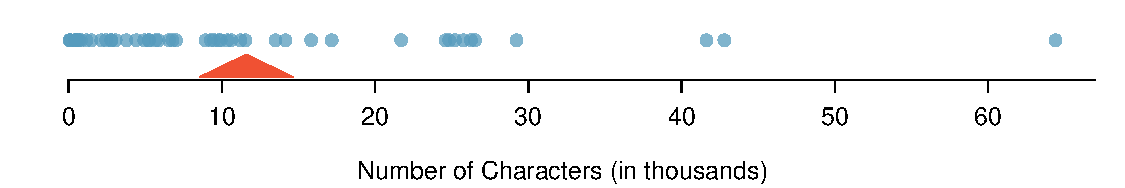
\includegraphics[width=\textwidth]{figures/emailCharactersDotPlot/emailCharactersDotPlot}
	   %\caption{A dot plot of num\_\hspace{0.3mm}char for the email50 data set.}
	   \label{emailCharactersDotPlot}
	\end{figure}
	\textbf{Stacked dot plot}
	\begin{figure}[h]
	   \small\centering
	 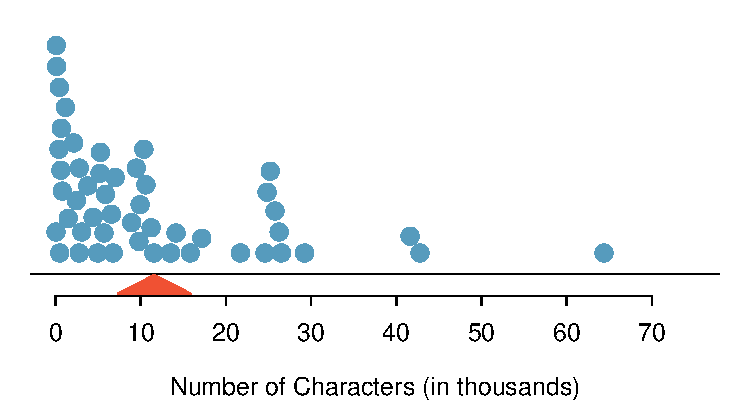
\includegraphics[width=0.7\textwidth]{figures/emailCharactersDotPlot/emailCharactersDotPlotStacked}
	   %\caption{A stacked dot plot of num\_\hspace{0.3mm}char for the email50 data set.}
	   \label{emailCharactersDotPlotStacked}
	\end{figure}	
\end{frame}
\begin{frame}{Mean}
	
The \textbf{mean}, sometimes called the \textbf{average}, is a common way to measure the centre of a \textbf{distribution} of data. To find the mean number of characters in the 50 emails, we add up all the character counts and divide by the number of emails. 
	\begin{eqnarray*}
	\bar{x} = \frac{21.7 + 7.0 + \cdots + 15.8}{50} = 11.6
	\end{eqnarray*}
	\begin{figure}[h]
	   \small\centering
	 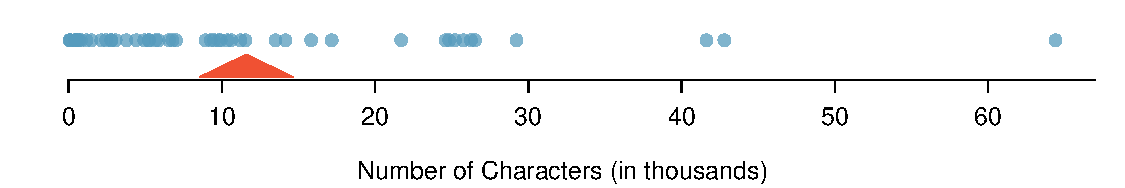
\includegraphics[width=\textwidth]{figures/emailCharactersDotPlot/emailCharactersDotPlot}
	   %\caption{A stacked dot plot of num\_\hspace{0.3mm}char for the email50 data set.}
	   \label{emailCharactersDotPlotStacked}
	\end{figure}
\end{frame}
\begin{frame}{Mean}
\begin{framed}
	The \textbf{sample mean} of a numerical variable is computed as the sum of all of the observations divided by the number of observations:
	\begin{eqnarray*}
	\bar{x} = \frac{x_1+x_2+\cdots+x_n}{n}
	\end{eqnarray*}
	where $x_1, x_2, \dots, x_n$ represent the $n$ observed values.
\end{framed}
\end{frame}
\begin{frame}{Histograms}
\textbf{Bins/Frequency}
	
\vspace{1cm}	
\small\begin{tabular}{l ccc ccc ccc c}
		  \hline
		Characters & \\
		(in thousands) & \raisebox{1.5ex}[0pt]{0-5} & \raisebox{1.5ex}[0pt]{5-10} & \raisebox{1.5ex}[0pt]{10-15} & \raisebox{1.5ex}[0pt]{15-20} & \raisebox{1.5ex}[0pt]{20-25} &  \raisebox{1.5ex}[0pt]{$\cdots$} & \raisebox{1.5ex}[0pt]{60-65} \\
		  \hline
		Count & 19 & 12 & 6 & 2 & 3 & $\cdots$ & 1 \\
		  \hline
\end{tabular}
\begin{figure}[bth]
   \centering
   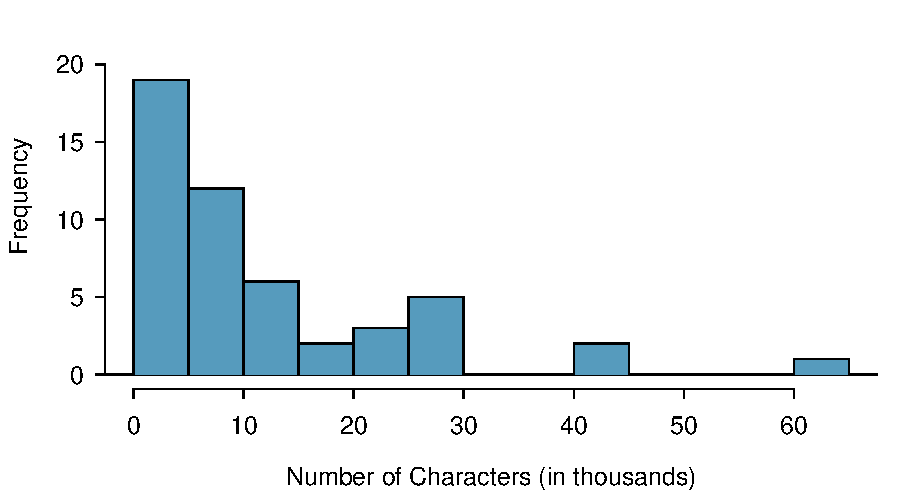
\includegraphics[width=0.72\textwidth]{figures/email50NumCharHist/email50NumCharHist}
   %\caption{A histogram of \var{num\_\hspace{0.3mm}char}. This distribution is very strongly skewed to the right.\index{skew!example: very strong}}
   %\label{email50NumCharHist}
\end{figure}
		%\caption{The counts for the binned num\_\hspace{0.3mm}char data.}
		%\label{binnedNumCharTable}
	
		
\end{frame}
\begin{frame}{Characteristics of Histograms-Skew}
	\textbf{Skew:} When data trail off in one direction, the distribution has a \textbf{long tail}.
	\begin{itemize}
		\item If a distribution has a long left tail, it is \textbf{left skewed}. 
		\item If a distribution has a long right tail, it is \textbf{right skewed}. 
		\item Data sets that show roughly equal trailing off in both directions are called \textbf{symmetric}.
	\end{itemize}
	\begin{figure}
	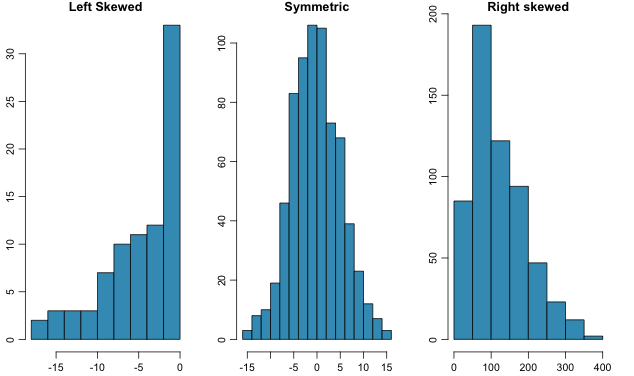
\includegraphics[width=0.8\textwidth]{figures/Skewed}
	\end{figure}
\end{frame}
\begin{frame}{Characteristics of Histograms-Modes}
	\textbf{Modes:} A \textbf{mode} is represented by a prominent peak in the distribution.
	\begin{itemize}
		\item \textbf{unimodal}
		\item \textbf{bimodal}
		\item \textbf{multimodal}
	\end{itemize}
	\begin{figure}[h]
	   \centering
	   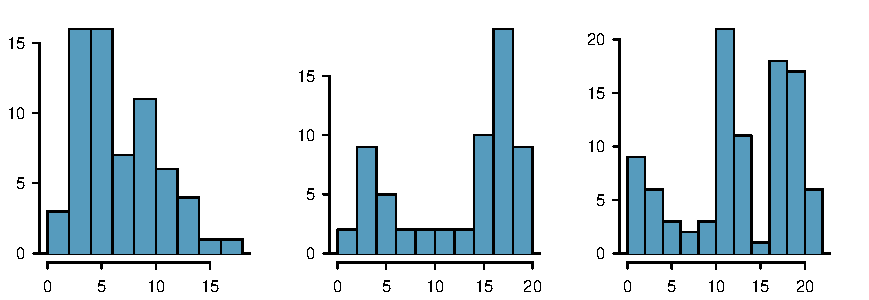
\includegraphics[width=\textwidth]{figures/singleBiMultiModalPlots/singleBiMultiModalPlots}
	  % \caption{Counting only prominent peaks, the distributions are (left to right) unimodal, bimodal, and multimodal.}
	   \label{singleBiMultiModalPlots}
	\end{figure}
\end{frame}
\begin{frame}{Deviation}
\begin{figure}[h]
	   \centering
	   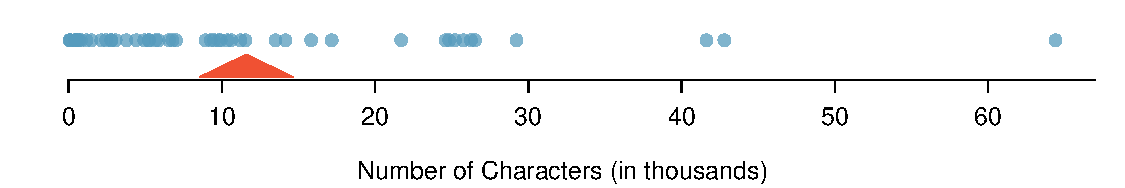
\includegraphics[width=\textwidth]{figures/emailCharactersDotPlot/emailCharactersDotPlot}
	   %\caption{A dot plot of num\_\hspace{0.3mm}char for the email50 data set.}
	   \label{emailCharactersDotPlot}
	\end{figure}
\end{frame}

\begin{frame}{Variance and standard deviation}
\small	\begin{framed}
	\textbf{Deviation} of observation $i$ is the distance of an observation from its mean, $x_i-\bar{x}$.
	\end{framed}
	
	\begin{framed}
		The \textbf{sample variance}, $s^2$, of a numerical variable is computed as the sum of the squared deviation all of the observations divided by the number of observations minus one:
		\begin{equation*}
		s^2 = \frac{(x_1-\bar{x})^2+(x_2-\bar{x})^2+\cdots+(x_n-\bar{x})^2}{n-1}
		\end{equation*}
		where $x_1, x_2, \dots, x_n$ represent the $n$ observed values.
		\end{framed}
		
		\begin{framed}
	The \textbf{standard deviation}, s, is defined as the square root of the variance.
	\end{framed}
\end{frame}
\begin{frame}
	\begin{figure}
	\centering
	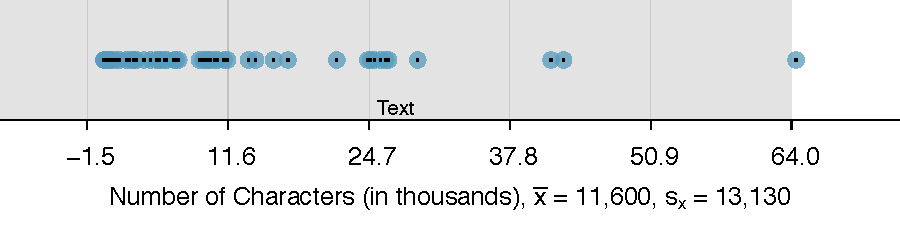
\includegraphics[width=\textwidth]{figures/sdAsRuleForEmailNumChar/sdAsRuleForEmailNumChar}
	
	\label{sdAsRuleForEmailNumChar}
	\end{figure}
	In the num\_\hspace{0.3mm}char data, 41 of the 50 emails (82\%) are within 1~standard deviation of the mean, and 47 of the 50 emails (94\%) are within 2 standard deviations.
\end{frame}
\begin{frame}{Is it enough?}
	Three very different population distributions with the same sample mean $\bar{x}=0$ and standard deviation $s=1$.
	\begin{figure}
	\centering
	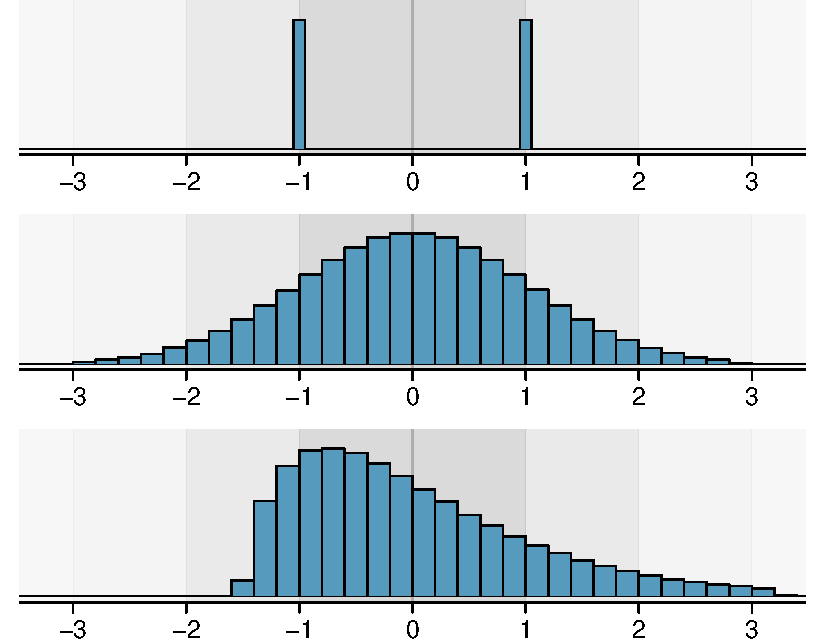
\includegraphics[width=0.63\textwidth]{figures/severalDiffDistWithSdOf1/severalDiffDistWithSdOf1}
	%\caption{Three very different population distributions with the same mean $\mu=0$ and standard deviation $\sigma=1$.}
	\label{severalDiffDistWithSdOf1}
	\end{figure}
\end{frame}
\begin{frame}{Boxplot}

	\begin{figure}[h]
	   \centering
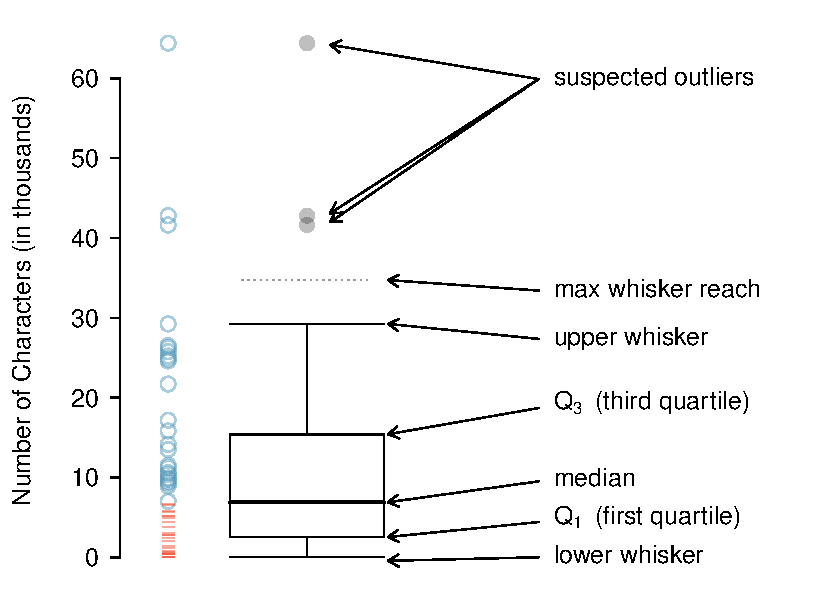
\includegraphics[width=0.7\textwidth]{figures/boxPlotLayoutNumVar/boxPlotLayoutNumVar}
\small\caption{A vertical dot plot next to a labelled box plot for the number of characters in 50 emails. The median (6,890), splits the data into the bottom 50\% and the top 50\%, marked in the dot plot by horizontal dashes and open circles, respectively.}
\end{figure}
\end{frame}
\begin{frame}{Median-IQR-Whiskers}
\small\begin{framed}If the data are ordered from smallest to largest, the \textbf{median} is the observation right in the middle. If there are an even number of observations, there will be two values in the middle, and the median is taken as their average.
\end{framed}	
\small\begin{framed}
	The \textbf{interquartile range} (IQR) is the length of the box in a box plot. It is computed as
	\begin{eqnarray*}
	IQR = Q_3 - Q_1
	\end{eqnarray*}
	where $Q_1$ and $Q_3$ are the $25^{th}$ and $75^{th}$ percentiles.
\end{framed}
\begin{framed}
\textbf{Whiskers} attempt to capture the data outside of the box, however, their reach is never allowed to be more than  $1.5\times IQR$.
\end{framed}
\end{frame}
\begin{frame}{Outliers}
\begin{framed}
	An \textbf{outlier} is an observation that appears extreme relative to the rest of the data.
\end{framed}	
\begin{framed}
	Examination of data for possible outliers serves many useful purposes, including\vspace{-2mm}
	\begin{enumerate}
	\item Identifying strong skew in the distribution.
	\item Identifying data collection or entry errors. For instance, we re-examined the email purported to have 64,401 characters to ensure this value was accurate.
	\item Providing insight into interesting properties of the data.\vspace{0.5mm}
	\end{enumerate}
\end{framed}
\end{frame}
\begin{frame}{Robust statistics}
	\begin{figure}[ht]
	\centering
	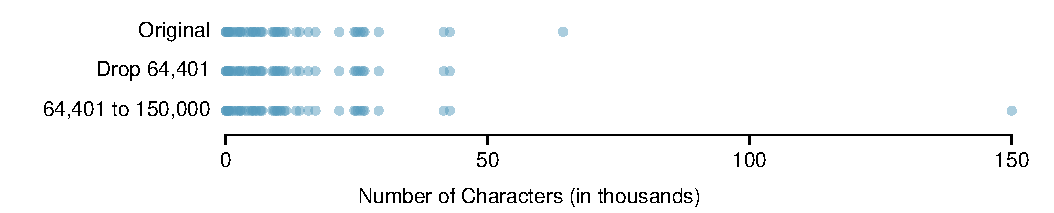
\includegraphics[width=\textwidth]{figures/email50NumCharDotPlotRobustEx/email50NumCharDotPlotRobustEx}
	%\caption{Dot plots of the original character count data and two modified data sets.}
	\label{email50NumCharDotPlotRobustEx}
	\end{figure}


\resizebox{0.9\textwidth}{!}{
	\begin{tabular}{l c cc c cc}
	  \hline
	& \hspace{0mm} & \multicolumn{2}{c}{\bf robust} & \hspace{2mm} & \multicolumn{2}{c}{\bf not robust} \\
	scenario && median & IQR && $\bar{x}$ & $s$ \\ 
	  \hline
	original num\_\hspace{0.3mm}char data 	&& 6,890 & 12,875 && 11,600 & 13,130 \\
	
	drop 66,924 observation		&& 6,768 & 11,702 && 10,521 & 10,798 \\
	
	move 66,924 to 150,000		&& 6,890 & 12,875 && 13,310 & 22,434 \\
	   \hline
	\end{tabular}}


\end{frame}
\begin{frame}{Data Transformation}
\begin{figure}
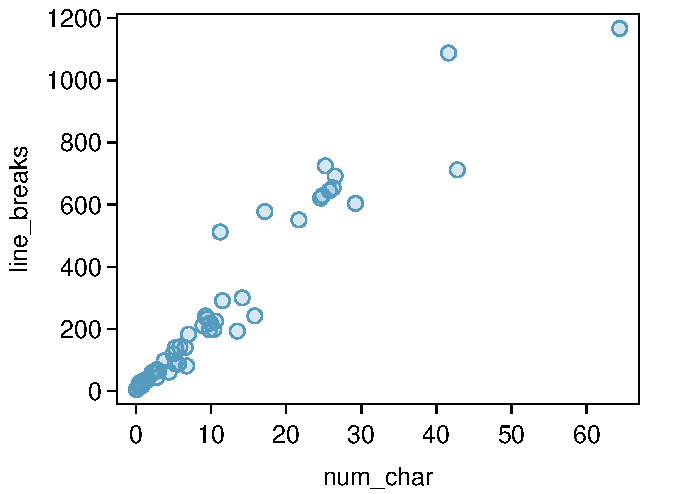
\includegraphics[width=0.44\textwidth]{figures/email50LinesCharactersMod/email50LinesCharactersMod}
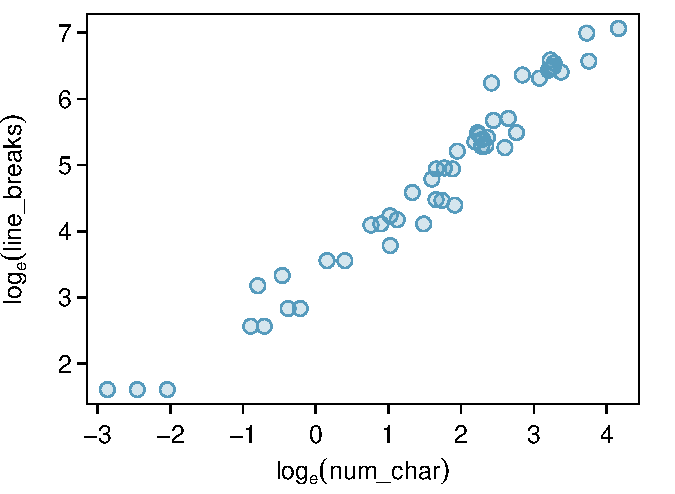
\includegraphics[width=0.44\textwidth]{figures/email50LinesCharactersMod/email50LinesCharactersModLog}
\end{figure}
\textbf{Common transformation functions}
\begin{itemize}
\item $log(x)$
\item $\sqrt{x}$
\item $\frac{1}{x}$
\end{itemize}
\end{frame}
\begin{frame}{Categorical Data I}
\textbf{Summary table}
\begin{table}[htb]
	\centering
	\resizebox{0.5\textwidth}{!}{
	\begin{tabular}{cccc}
	& & \textbf{number}&\\
	  \hline
	none & small & big & Total \\ 
	 % \hline
	 549 & 2827 & 545 & 3921 \\
	   \hline
	\end{tabular}}
	\end{table}
	A table that summarises data for a categorical variable is called a \textbf{frequency table.}
	\begin{table}[htb]
	\centering
	\resizebox{0.7\textwidth}{!}{
	\begin{tabular}{cccc}
	& & \textbf{number}&\\
	  \hline
	none & small & big & Total \\ 
	 % \hline
	$\frac{549}{3921}=0.14$ & $\frac{2827}{3921}=0.72$ & $\frac{545}{3921}=0.14$ & $1.00$ \\
	   \hline
	\end{tabular}}
	\end{table}
		
\end{frame}
\begin{frame}{Barplot}
	\begin{figure}[bht]
	   \centering
	   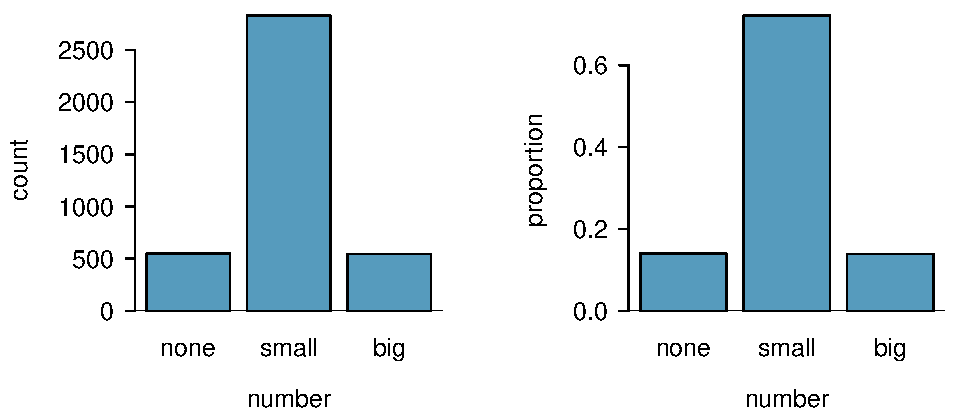
\includegraphics[height=2in]{figures/emailNumberBarPlot/emailNumberBarPlot}
	   \caption{Two bar plots of number. The left panel shows the counts, and the right panel shows the proportions in each group.}
	   \label{emailNumberBarPlot}
	\end{figure}
\end{frame}
\begin{frame}{Categorical Data II}
A table that 
	summarises data for two categorical variables in this way is called a \textbf{contingency table}.
	
	
	\begin{table}[ht]
	\centering
	\resizebox{0.7\textwidth}{!}{
	\begin{tabular}{ll  ccc  rr}
	& & \multicolumn{3}{c}{\bf number} & \\
	  \cline{3-5}
	& & none & small & big & Total & \hspace{2mm}\  \\ 
	  \cline{2-6}
		 & spam &  149 & 168 &  50 & 367 \\ 
	\raisebox{1.5ex}[0pt]{spam} 
		& not spam &  400 & 2659 & 495 & 3554 \\ 
	  \cline{2-6}
	& Total & 549 & 2827 & 545 & 3921 \\
	  \cline{2-6}
	\end{tabular}}
	\label{emailSpamNumberTableTotals}
	%library(openintro); library(xtable); data(email); tab <- table(email[,c("spam", "number")])[2:1,]; xtable(tab); rowSums(tab); colSums(tab); sum(tab)
	\end{table}
	
	\textbf{A contingency table with row proportions}
	\begin{table}[l]
		\resizebox{1\textwidth}{!}{
	\begin{tabular}{l rrr r}
	  \hline
	 & none & small & big & Total \\ 
	  \hline
	spam &  $\frac{149}{367} = 0.406$ & $\frac{168}{367} = 0.458$ &
				$\frac{50}{367} = 0.136$ & 1.000 \\ 
	not spam &  $\frac{400}{3554} = 0.113$ & $\frac{2657}{3554} = 0.748$ &
				$\frac{495}{3554} = 0.139$ & 1.000 \\ 
	   \hline
	Total & $\frac{549}{3921} = 0.140$ & $\frac{2827}{3921} = 0.721$ &
				$\frac{545}{392} = 0.139$ & 1.000 \\
	  \hline
	\end{tabular}}
	
	\end{table}

\end{frame}
\begin{frame}{Segmented bar plot}
	A \textbf{segmented barplot} is a graphical display of contingency table information.
	\begin{figure}
	 	\centering
		\begin{minipage}{.5\textwidth}
		  \centering
	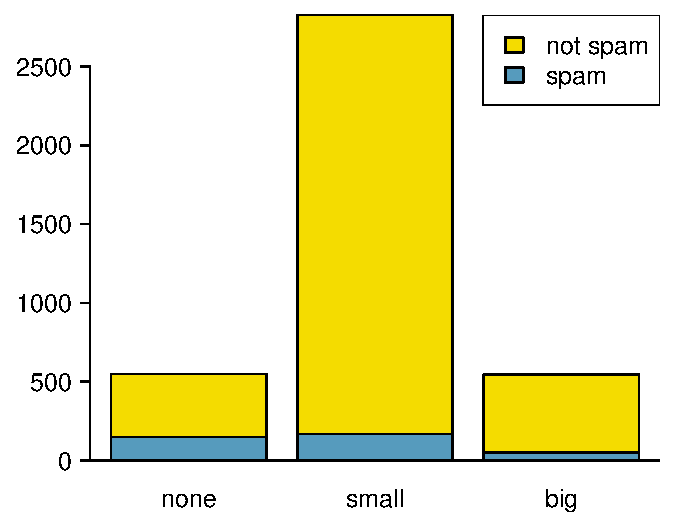
\includegraphics[width=\textwidth]{figures/emailSpamNumberSegBar/emailSpamNumberSegBar}
	\end{minipage}%
	\begin{minipage}{.5\textwidth}
	  \centering
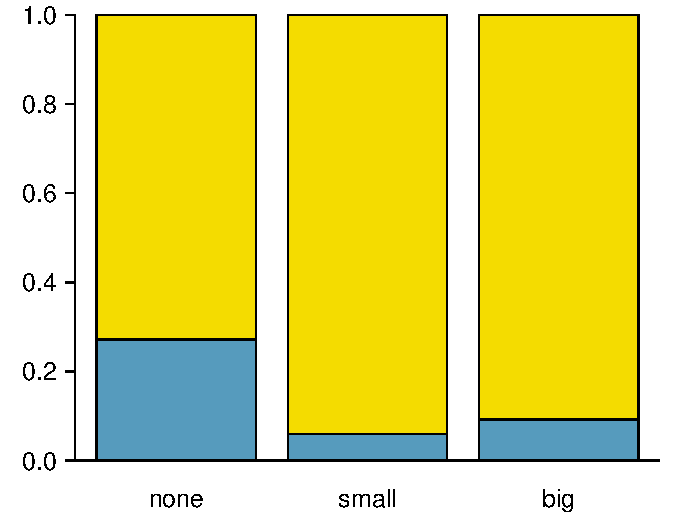
\includegraphics[width=\textwidth]{figures/emailSpamNumberSegBar/emailSpamNumberSegBarSta}
\label{emailSpamNumberSegBarSta}
\end{minipage}
\end{figure}
\end{frame}
\begin{frame}{Categorical II}
	\textbf{A contingency table with column proportions}
	\begin{table}[ht]
	\resizebox{\textwidth}{!}{
	\begin{tabular}{l rrr r}
	  \hline
	 & none & small & big & Total \\ 
	  \hline
	spam &  $149/549 = 0.271$ & $168/2827 = 0.059$ &
					$50/545 = 0.092$ & $367/3921 = 0.094$ \\ 
	not spam &  $400/549 = 0.729$ & $2659/2827 = 0.941$ &
					$495/545 = 0.908$ & $3684/3921 = 0.906$ \\ 
	   \hline
	Total & 1.000 & 1.000 & 1.000 & 1.000 \\
	   \hline
	\end{tabular}}
	
	% library(openintro); data(email); g <- table(email$spam, email$number)[2:1,]; g / rep(colSums(g), rep(2, 3)); g; colSums(g)
	\end{table}
\end{frame}
\begin{frame}{Mosaic plot}
	A mosaic plot is a graphical display that allows you to examine the relationship among two or more categorical variables. 
	\begin{enumerate}
	\item 	The mosaic plot is a square with length one. 
	\item The horizontal bars  widths are proportional to the probabilities associated with the first 
	categorical variable. 
	\item The vertical  bars widths are proportional to the 
	conditional probabilities of the second categorical variable. 
	\end{enumerate}
	
\end{frame}
\begin{frame}{Mosaic Plots}
		\begin{figure}
		 	\centering
			\begin{minipage}{.5\textwidth}
			  \centering
		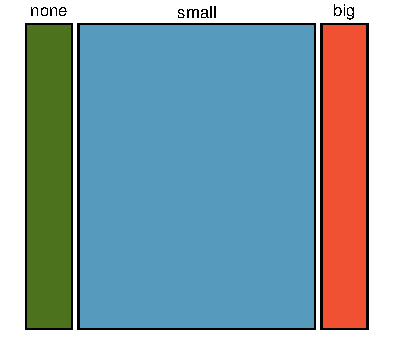
\includegraphics[width=\textwidth]{figures/emailSpamNumberMosaicPlot/emailNumberMosaic}
		\end{minipage}%
		\begin{minipage}{.5\textwidth}
		  \centering
	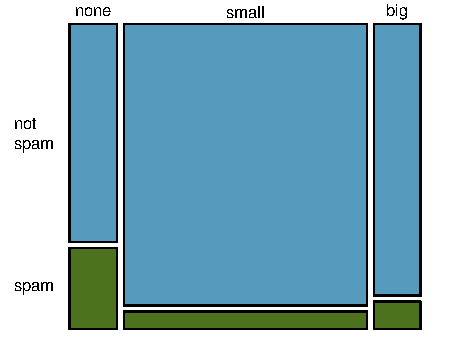
\includegraphics[width=\textwidth]{figures/emailSpamNumberMosaicPlot/emailSpamNumberMosaic}
	\label{emailSpamNumberSegBarSta}
	\end{minipage}
	\end{figure}

\end{frame}
\begin{frame}{Comparing numerical data across groups 
}
\begin{figure}
   \centering
   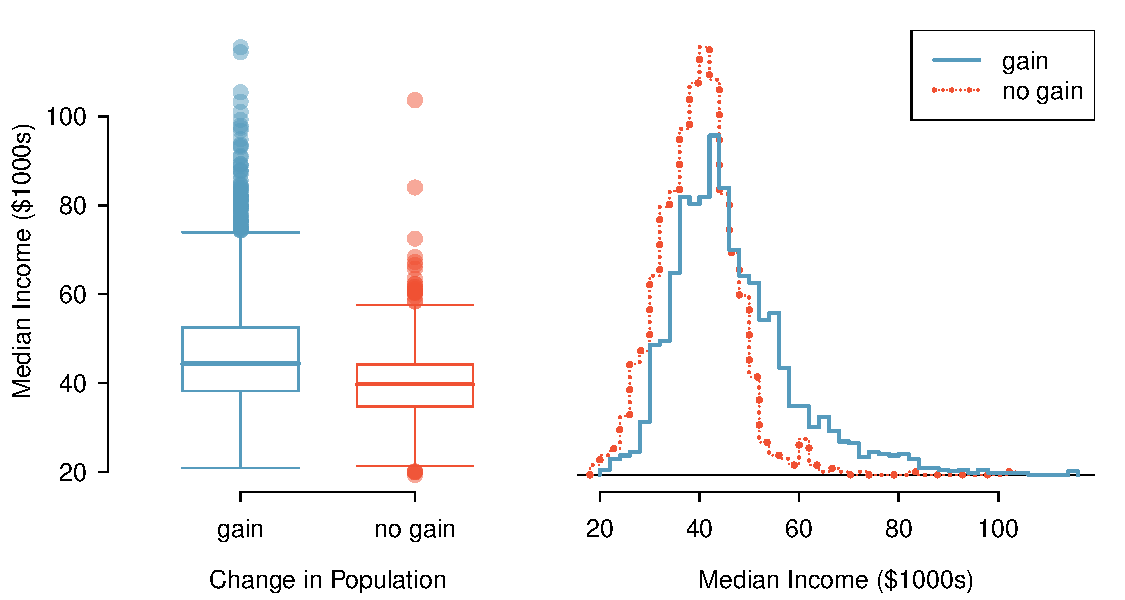
\includegraphics[width=\textwidth]{figures/countyIncomeSplitByPopGain/countyIncomeSplitByPopGain}
   %\caption{Side-by-side box plot (left panel) and hollow histograms (right panel) for med\_\hspace{0.3mm}income, where the counties are split by whether there was a population gain or loss from 2000 to 2010. The income data were collected between 2006 and 2010.}
 %  \label{countyIncomeSplitByPopGain}
\end{figure}
\end{frame}
\begin{frame}{Some probability}
\textbf{Common Probability distributions}
\begin{itemize}
\item Normal distribution
\item Bernoulli
\item Geometric distribution
\item Binomial distribution
\end{itemize}
\end{frame}
\begin{frame}{Normal Distribution}
	\begin{figure}
	 	\centering
		\begin{minipage}{.5\textwidth}
		  \centering
	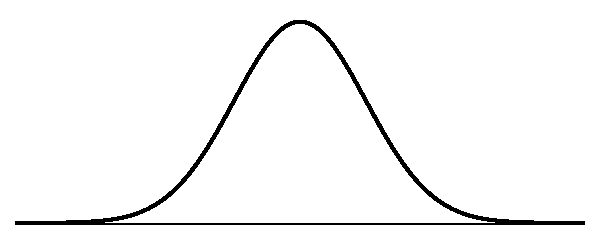
\includegraphics[width=\textwidth]{figures/simpleNormal/simpleNormal}
	\end{minipage}%
	\begin{minipage}{\textwidth}
	  \begin{itemize}
		\item $X\sim \mathcal{N}(\mu,\sigma^2)$
		\item Probability density 
		function:

		$f(x,\mu,\sigma)=\frac{1}{\sigma\sqrt{2\pi}}e^{-\frac{(x-\mu)^2}{2\sigma^2}}$
		\item Parameters:
		\begin{itemize}
			\item $\mu$ denotes the mean
			\item $\sigma^2$ denotes the variance\footnote{ $\sigma$ denotes the standard deviation}
		\end{itemize}
		\end{itemize}
\end{minipage}
\end{figure}
\end{frame}
\begin{frame}{Normal Distribution}
	\begin{figure}[hht]
	\centering
	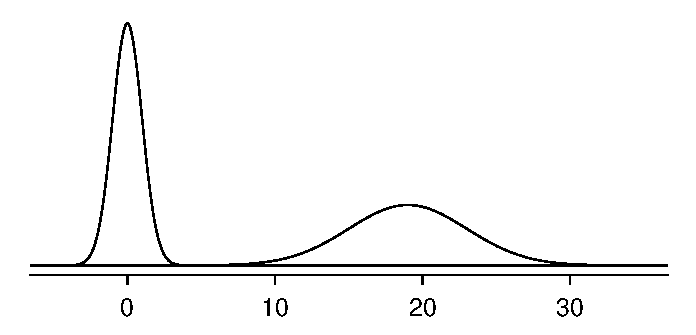
\includegraphics[width=0.62\textwidth]{figures/twoSampleNormalsStacked/twoSampleNormalsStacked}
	\end{figure}
	\begin{align*}
	N(\mu=0,\sigma=1)\quad\text{and}\quad N(\mu=19,\sigma=4)
	\end{align*}
\end{frame}
\begin{frame}{Score comparison}
	
	\begin{figure}
	 	\centering
		\begin{minipage}{.7\textwidth}
		  \centering
	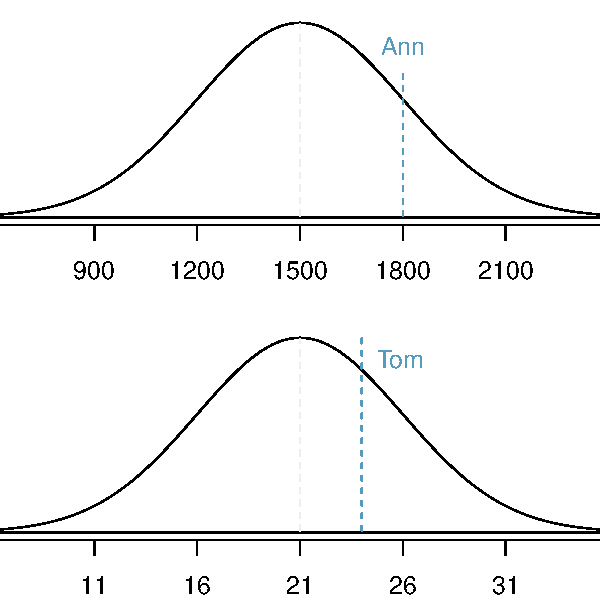
\includegraphics[width=0.8\textwidth]{figures/satActNormals/satActNormals}
	\end{minipage}%
	\begin{minipage}{0.3\textwidth}
	  \small \begin{itemize}
	 \item SAT follow $\mathcal{N}(1500,300)$\\
	\item ACT follow $\mathcal{N}(21,5)$
\end{itemize}
\end{minipage}
	\end{figure}
\end{frame}
\begin{frame}{Standardizing with Z scores 
}
\begin{framed}
The \textbf{Z score} of an observation is the number of standard deviations it falls above or below the mean. We compute the Z score for an observation $x$ that follows a distribution with mean $\mu$ and standard deviation $\sigma$ using
\begin{eqnarray*}
Z = \frac{x-\mu}{\sigma}
\end{eqnarray*}
\end{framed}

\end{frame}

\begin{frame}{Score comparison}
	
	\begin{figure}
	 	\centering
		\begin{minipage}{.5\textwidth}
		  \centering
	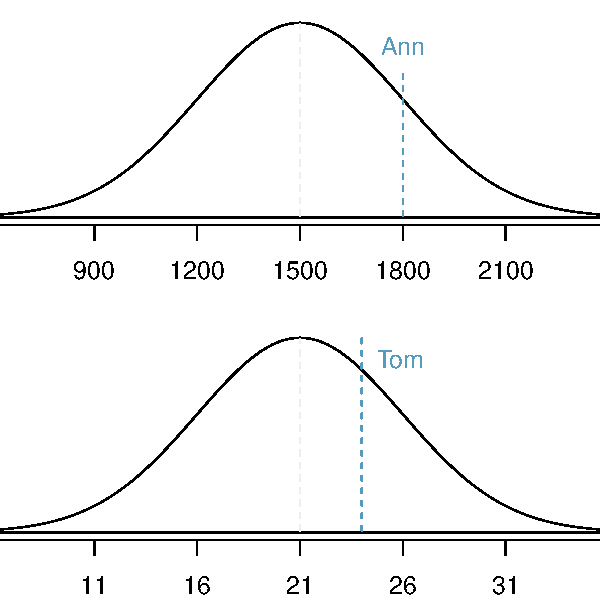
\includegraphics[width=0.8\textwidth]{figures/satActNormals/satActNormals}
	\end{minipage}%
	\begin{minipage}{0.7\textwidth}
	  \small \begin{itemize}
	 \item $Z_{Ann} = \frac{x_{Ann} - \mu_{SAT}}{\sigma_{SAT}}= 1$

	\vspace{2cm}
	\item $Z_{Tom} = \frac{x_{Tom} - \mu_{ACT}}{\sigma_{ACT}} = 0.6$
\end{itemize}
\end{minipage}
	\end{figure}
\end{frame}
\begin{frame}{Percentile}
	\begin{itemize}
		\item What percentile does Ann fall  among all 
		SAT test-takers? 
		\item Ann’s \textbf{percentile} is the percentage of people who earned a lower SAT score than her. Ann is in the $84th$ percentile of SAT takers.
	\end{itemize}
		\begin{figure}[htb]
		   \centering
		   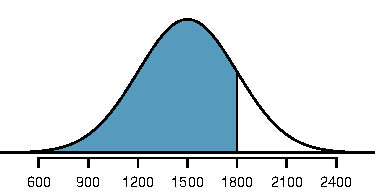
\includegraphics[height=1.5in]{figures/satBelow1800/satBelow1800}
		   
		\end{figure}
\end{frame}
\begin{frame}{Normal probability table}
	\begin{table}
	\centering
	\resizebox{1\textwidth}{!}{
	\begin{tabular}{c | rrrrr | rrrrr |}
	  \cline{2-11}
	&&&& \multicolumn{4}{c}{Second decimal place of $Z$} &&& \\
	  \cline{2-11}
	$Z$ & 0.00 & 0.01 & 0.02 & 0.03 & 0.04 & 0.05 & 0.06 & 0.07 & 0.08 & 0.09 \\
	  \hline
	  \hline
	0.0 & \scriptsize{0.5000} & \scriptsize{0.5040} & \scriptsize{0.5080} & \scriptsize{0.5120} & \scriptsize{0.5160} & \scriptsize{0.5199} & \scriptsize{0.5239} & \scriptsize{0.5279} & \scriptsize{0.5319} & \scriptsize{0.5359} \\
	  0.1 & \scriptsize{0.5398} & \scriptsize{0.5438} & \scriptsize{0.5478} & \scriptsize{0.5517} & \scriptsize{0.5557} & \scriptsize{0.5596} & \scriptsize{0.5636} & \scriptsize{0.5675} & \scriptsize{0.5714} & \scriptsize{0.5753} \\
	  0.2 & \scriptsize{0.5793} & \scriptsize{0.5832} & \scriptsize{0.5871} & \scriptsize{0.5910} & \scriptsize{0.5948} & \scriptsize{0.5987} & \scriptsize{0.6026} & \scriptsize{0.6064} & \scriptsize{0.6103} & \scriptsize{0.6141} \\
	%  May comment out 0.0-0.2 to make extra space. Then insert the following line:
	%  $\vdots$ &   $\vdots$ &   $\vdots$ &   $\vdots$ &   $\vdots$ &   $\vdots$ &   $\vdots$ &   $\vdots$ &   $\vdots$ &   $\vdots$ &   $\vdots$ \\
	  0.3 & \scriptsize{0.6179} & \scriptsize{0.6217} & \scriptsize{0.6255} & \scriptsize{0.6293} & \scriptsize{0.6331} & \scriptsize{0.6368} & \scriptsize{0.6406} & \scriptsize{0.6443} & \scriptsize{0.6480} & \scriptsize{0.6517} \\
	0.4 & \scriptsize{0.6554} & \scriptsize{0.6591} & \scriptsize{0.6628} & \scriptsize{0.6664} & \scriptsize{0.6700} & \scriptsize{0.6736} & \scriptsize{0.6772} & \scriptsize{0.6808} & \scriptsize{0.6844} & \scriptsize{0.6879} \\
	  \hline
	  0.5 & \scriptsize{0.6915} & \scriptsize{0.6950} & \scriptsize{0.6985} & \scriptsize{0.7019} & \scriptsize{0.7054} & \scriptsize{0.7088} & \scriptsize{0.7123} & \scriptsize{0.7157} & \scriptsize{0.7190} & \scriptsize{0.7224} \\
	  0.6 & \scriptsize{0.7257} & \scriptsize{0.7291} & \scriptsize{0.7324} & \scriptsize{0.7357} & \scriptsize{0.7389} & \scriptsize{0.7422} & \scriptsize{0.7454} & \scriptsize{0.7486} & \scriptsize{0.7517} & \scriptsize{0.7549} \\
	  0.7 & \scriptsize{0.7580} & \scriptsize{0.7611} & \scriptsize{0.7642} & \scriptsize{0.7673} & \scriptsize{0.7704} & \scriptsize{0.7734} & \scriptsize{0.7764} & \scriptsize{0.7794} & \scriptsize{0.7823} & \scriptsize{0.7852} \\
	0.8 & \scriptsize{0.7881} & \scriptsize{0.7910} & \scriptsize{0.7939} & \scriptsize{0.7967} & \scriptsize{0.7995} & \scriptsize{0.8023} & \scriptsize{0.8051} & \scriptsize{0.8078} & \scriptsize{0.8106} & \scriptsize{0.8133} \\
	  0.9 & \scriptsize{0.8159} & \scriptsize{0.8186} & \scriptsize{0.8212} & \scriptsize{0.8238} & \scriptsize{0.8264} & \scriptsize{0.8289} & \scriptsize{0.8315} & \scriptsize{0.8340} & \scriptsize{0.8365} & \scriptsize{0.8389} \\
	  \hline
	  \hline
	  1.0 & \textbf{0.8413} & \scriptsize{0.8438} & \scriptsize{0.8461} & \scriptsize{0.8485} & \scriptsize{0.8508} & \scriptsize{0.8531} & \scriptsize{0.8554} & \scriptsize{0.8577} & \scriptsize{0.8599} & \scriptsize{0.8621} \\
	  1.1 & \scriptsize{0.8643} & \scriptsize{0.8665} & \scriptsize{0.8686} & \scriptsize{0.8708} & \scriptsize{0.8729} & \scriptsize{0.8749} & \scriptsize{0.8770} & \scriptsize{0.8790} & \scriptsize{0.8810} & \scriptsize{0.8830} \\
	  $\vdots$ &   $\vdots$ &   $\vdots$ &   $\vdots$ &   $\vdots$ &   $\vdots$ &   $\vdots$ &   $\vdots$ &   $\vdots$ &   $\vdots$ &   $\vdots$ \\
	   \hline
	\end{tabular}}
	\end{table}
\end{frame}
\begin{frame}{68-95-99.7 Rule\footnote{\small Otherwise know as the \textbf{three-sigma rule of thumb}}}
$68\%-95\%-99.7\%$ are, respectively, the probabilities for falling within 1, 2, and 3 standard deviations of the mean in a normal distribution.
	\begin{figure}[hht]
	\centering
	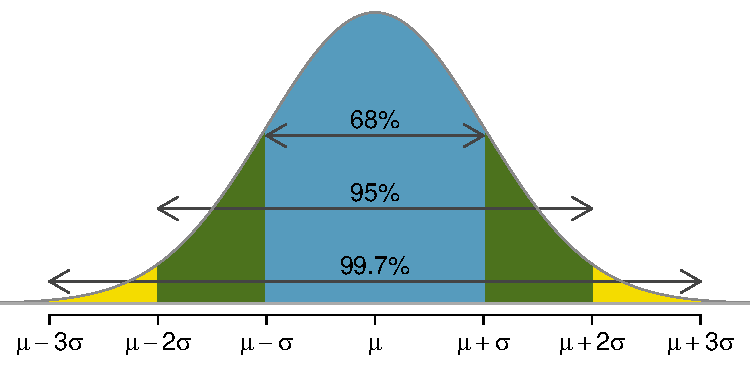
\includegraphics[height=1.7in]{figures/6895997/6895997}
	\end{figure}
\end{frame}
\begin{frame}{Evaluating the normal approximation}
\small	\begin{itemize}
		\item Best fitting normal curve
		\item Normal probability plot/ Quantile-quantile plot
	\end{itemize}
\end{frame}
\begin{frame}{Simulated normal distribution}
\small Histograms and normal probability plots for three simulated normal data sets; $n=40$ (left), $n=100$ (middle), $n=400$ (right).
	\begin{figure}
	\centering
	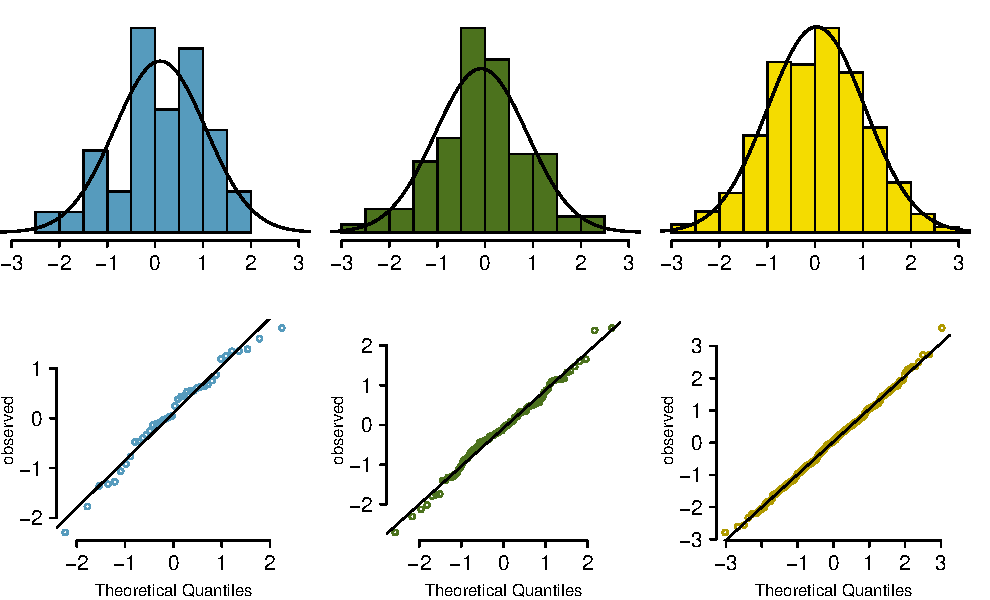
\includegraphics[width=\textwidth]{figures/normalExamples/normalExamples}
	\end{figure}
\end{frame}
\begin{frame}{NBA's players height}
We consider all 435 NBA players from the 2008-9 season.
\begin{figure}
\centering
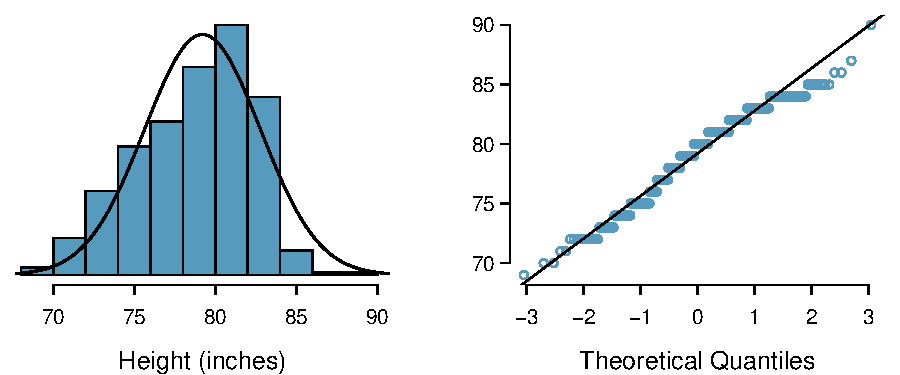
\includegraphics[width=\textwidth]{figures/nbaNormal/nbaNormal}

\end{figure}
\end{frame}	
\begin{frame}{Poker earnings}
	We consider the poker earnings of an individual over 50 days.\\
	Can we approximate poker winnings by a normal distribution?
	\begin{figure}
	\centering
	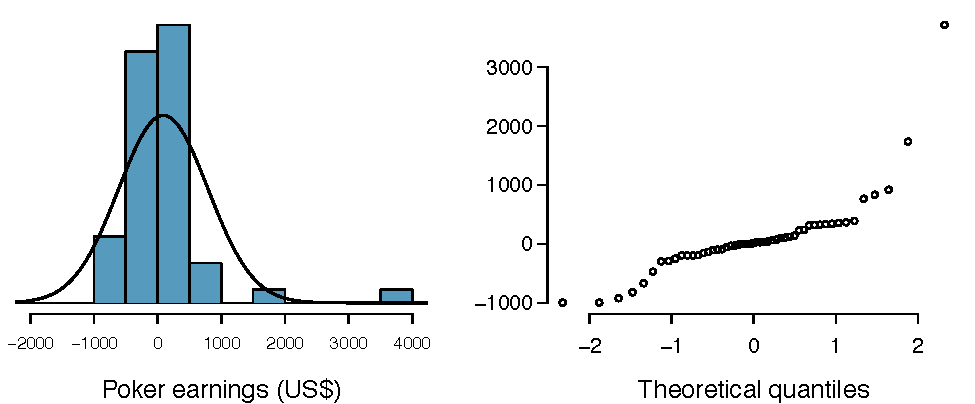
\includegraphics[width=\textwidth]{figures/pokerNormal/pokerNormal}
	%\caption{A histogram of poker data with the best fitting normal plot and a normal probability plot.}
	\end{figure}
\end{frame}
\begin{frame}{Bernoulli}
	
Consider a coin toss with outcome $\{H,T\}$ and the random variable $X:$
\[
X=\left\lbrace\begin{array}{lr}
1,&\text{for H (sucess)}\\
0,&\text{for T (failure)}
\end{array}\right.\]
	Then
	\[P(X=1)=P(\text{sucess})=p\] 
	 and 
	 \[P(X=0)=P(\text{fail})=1-p\]
	\end{frame}
	\begin{frame}{Bernoulli}
		\begin{framed}

		\textbf{Bernoulli random variable }\\
		If $X$ is a random variable that takes value 1 with probability of success $p$ and 0 with probability $1-p$, then $X$ is a Bernoulli random variable with mean and standard deviation
		\begin{align*}
		\mu &= p
			&\sigma&= \sqrt{p(1-p)}
		\end{align*}
	\end{framed}
\end{frame}
\begin{frame}{Geometric distribution}
\textbf{What is the probability of finding the first "success" after 4 trials? }

\[\{T,T,T,H\}\Rightarrow (1-p)^3p\]
\small\begin{framed}
		\textbf{Geometric distribution}\\
		Let $X$ is a random variable that takes the value $k$,  where $k$ is number of trial needed to get the first "sucess", then \vspace{-1mm}
\begin{eqnarray*}
P(X=k)=(1-p)^{k-1}p
\end{eqnarray*}
Additionally, the mean, variance, and standard deviation of the number of observed successes are\vspace{-2mm}
\begin{align*}
\mu &= \frac{1}{p}
	&\sigma^2 &= \frac{1-p}{p^2}
	&\sigma &= \sqrt{ \frac{1-p}{p^2}}
\label{binomialStats}
\end{align*}
\end{framed}



\end{frame}
\begin{frame}{Binomial distribution}
\textbf{Consider $3$ coin tosses, what is the probability of $2$ heads?}\\
Possible outcomes
\[(H,H,T)\quad (H,T,H)\quad (T,H,H),\]
with 
\[P((H,H,T))=p^2(1-p)\]
\[ P((H,T,H))=P((T,H,H))=p^2(1-p).\]
Then 

\[P(\text{'2 heads'})=3p^2(1-p)={3\choose 2}p^2(1-p)\]
\end{frame}
\begin{frame}{Binomial distribution} 
	
	
	
	\begin{framed}
		\textbf{Binomial distribution}\\
		Let $X$ is a random variable that takes the value $k$,  where $k$ is the number of  successes in $n$ independent trials, then \vspace{-1mm}
\begin{eqnarray*}
P(X=k)={n\choose k}p^k(1-p)^{n-k} = \frac{n!}{k!(n-k)!}p^k(1-p)^{n-k}
\end{eqnarray*}
Additionally, the mean, variance, and standard deviation of the number of observed successes are\vspace{-2mm}
\begin{align*}
\mu &= np
	&\sigma^2 &= np(1-p)
	&\sigma &= \sqrt{np(1-p)}
\label{binomialStats}
\end{align*}
\end{framed}
\end{frame}
\begin{frame}{Normal approximation to the binomial distribution-Graph}
	Hollow histograms of samples from the binomial model when $p=0.10$.
	\begin{figure}[h]
	\centering
	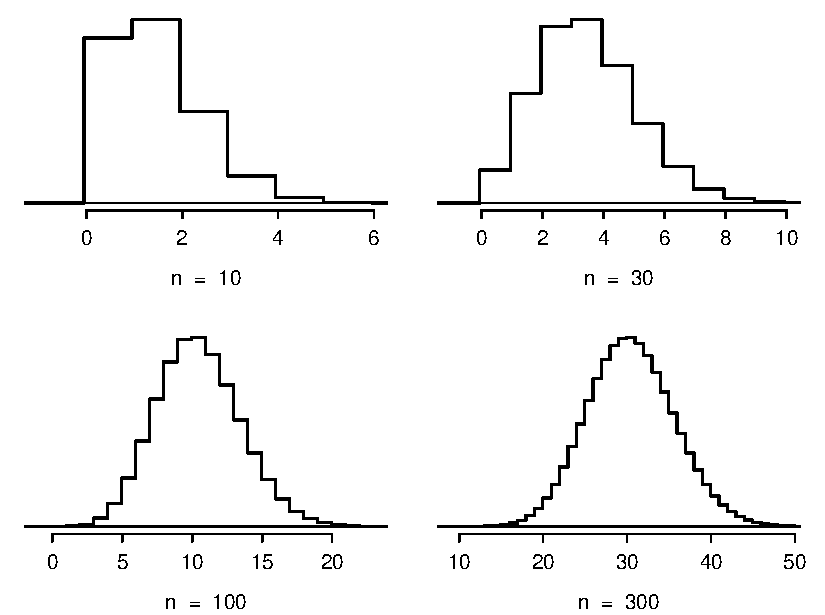
\includegraphics[width=0.8\textwidth]{figures/fourBinomialModelsShowingApproxToNormal/fourBinomialModelsShowingApproxToNormal}
	
	\end{figure}
\end{frame}
\begin{frame}{Normal approximation of the binomial distribution}
	\begin{framed}\textbf{Normal approximation of the binomial distribution}\\
The binomial distribution with probability of success $p$ is nearly normal when the sample size $n$ is sufficiently large that
\begin{enumerate}
	\item $np\geq 10,$ and
	\item $n(1-p)\geq 10$
	\end{enumerate} 
 The approximate normal distribution has parameters corresponding to the mean and standard deviation of the binomial distribution:\vspace{-1.5mm}
\begin{align*}
\mu &= np
&&\sigma= \sqrt{np(1-p)}
\end{align*}
\end{framed}
\end{frame}
\begin{frame}{Foundations for inference}
	\begin{itemize}
		\item A population
		\item Random sample
		\item \textbf{Statistical inference} is drawing conclusions based on the sample:
		\begin{enumerate}
			\item point estimates; the value of a particular variable
			\item an interval estimate; establishing confidence intervals for point estimates
			\item Hypothesis testing
		\end{enumerate} 
	\end{itemize}
\end{frame}
\begin{frame}{Inference on the population mean}
	\textbf{Q:} How sure are we that the estimated mean, $\bar{x}$, is near the true population mean, $\mu$?
\end{frame}
\begin{frame}{Data}
\small	Data in \textbf{run10}, all 16,924 runners who finished the 2012 Cherry Blossom 10 mile run in Washington, DC.
	\small
	\begin{table}[h]
	\centering
	\resizebox{0.6\textwidth}{!}{
	\begin{tabular}{rrrrr}
	  \hline
	ID & time & age & gender & state \\ 
	  \hline
	1 & 92.25 & 38.00 & M & MD \\ 
	2 & 106.35 & 33.00 & M & DC \\ 
	3 & 89.33 & 55.00 & F & VA \\ 
	4 & 113.50 & 24.00 & F & VA \\ 
	$\vdots$ & $\vdots$ & $\vdots$ & $\vdots$ & $\vdots$ \\
	16923 & 122.87 & 37.00 & F & VA \\ 
	16924 & 93.30 & 27.00 & F & DC \\ 
	   \hline
	\end{tabular}}
	\end{table}
	\begin{table}[h]
	\centering
	\resizebox{0.55\textwidth}{!}{
	\begin{tabular}{l p{65mm}}
	\hline
	{\bf variable} & {\bf description} \\
	\hline
	time & Ten mile run time, in minutes \\
	age & Age, in years \\
	gender & Gender (M for male, F for female) \\
	state & Home state (or country if not from the US) \\
	\hline
	\end{tabular}}
	\end{table}
\end{frame}
\begin{frame}{Sample}
	\textbf{run10Samp} a simple random sample of 100 runners from the 2012 Cherry Blossom Run.
	\begin{table}
	\centering
	\resizebox{0.55\textwidth}{!}{
	\begin{tabular}{rrrrr}
	  \hline
	ID & time & age & gender & state \\ 
	  \hline
	1983 & 88.31 & 59 & M & MD \\ 
	8192 & 100.67 & 32 & M & VA \\ 
	11020 & 109.52 & 33 & F & VA \\ 
	  $\vdots$ &   $\vdots$ &   $\vdots$ &   $\vdots$ &   $\vdots$ \\ 
	1287 & 89.49 & 26 & M & DC \\ 
	   \hline
	\end{tabular}}
	\end{table}
	\small To estimate the average 10 mile run time of all participants, take the average time for the sample:
	\begin{eqnarray*}
	\bar{x} = \frac{88.22 + 100.58 + \dots + 89.40}{100} = 95.61
	\end{eqnarray*}
\end{frame}
\begin{frame}{Population parameters vs. Point estimates}
	\begin{table}[h]
	\centering
	\resizebox{0.55\textwidth}{!}{
	\begin{tabular}{ l rr}
	\hline
	time		& estimate & parameter  \\
	\hline
	mean		& 95.61 & 94.52 \\
	median	& 95.46 & 94.03 \\
	st. dev.		& 15.78 & 15.93 \\
	\hline
	\end{tabular}}
	\end{table}
\end{frame}
\begin{frame}{Running mean}
	A \textbf{running mean is} a sequence of means, where each mean uses one more observation in 
	its calculation than the mean directly before it in the sequence.
	\begin{figure}
	   \centering
	   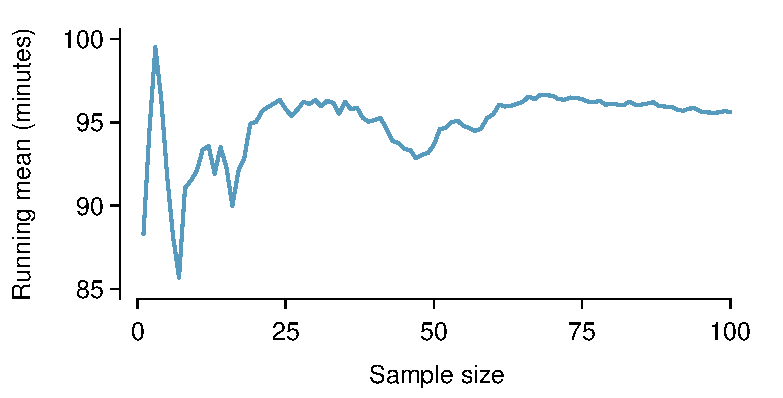
\includegraphics[width=0.7\textwidth]{figures/netTimeRunningMean/netTimeRunningMean}
	\end{figure}
\small\textbf{Note:} The mean tends to approach the true population average as more data become available.
\end{frame}
\begin{frame}{Sampling distribution}
	Take 1000 random samples of 100 individuals from \textbf{run10}, with estimated average time:
	\begin{figure}
	 	\centering
		\begin{minipage}{.5\textwidth}
		  \centering\begin{table}[h]
	\centering
	\resizebox{0.65\textwidth}{!}{
	\begin{tabular}{ l r}
	\hline
	Sample		& estimated average  \\
	\hline
	1		& 95.61 \\
	2	& 93.43\\
	3		&  93.43 \\
	\vdots\\
	1000 & 94.16\\
	\hline
	\end{tabular}}
	\end{table}
\end{minipage}%
\begin{minipage}{.65\textwidth}\centering
   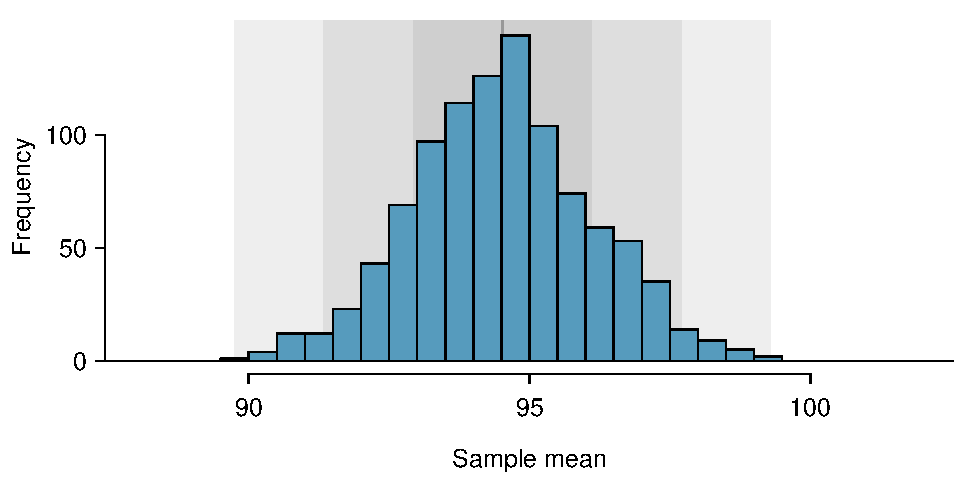
\includegraphics[width=0.85\textwidth]{figures/netTime1000SamplingDistribution/netTime1000SamplingDistribution}
\end{minipage}
\end{figure}
\end{frame}
\begin{frame}{Sampling distribution}
	\begin{itemize}
		\item The sampling distribution represents the distribution of the point estimates based on samples of a fixed size from a certain population.
		\item Uncertainty about the estimate is captured by the standard deviation of the estimate, called the \textbf{standard error (SE)}.
			\item \textit{Computing SE for the sample mean:}
			Given $n$ independent observations from a population with standard deviation $\sigma$, the standard error of the sample mean is equal to \vspace{-1mm}
			\begin{eqnarray}
			SE = \frac{\sigma}{\sqrt{n}}
			\label{seOfXBar}
			\end{eqnarray}
	\end{itemize}
\end{frame}
\begin{frame}{Confidence interval }
	\centering
	A plausible range of values for the population parameter is called a \textbf{confidence interval}.
\end{frame}
\begin{frame}{An approximate 95\% confidence interval 
}
 
	 

	\begin{itemize}
		\item The standard error represents the standard deviation associated with the estimate.
		\item Roughly 95\% of the time the estimate will be within 2 standard errors of the parameter.
		\item If the interval spreads out 2 standard errors from the point estimate, we can be roughly 
		95\% confident that we have captured the true parameter:
		\begin{eqnarray*}
		\text{point estimate}\ \pm\ 2\times SE
		\end{eqnarray*}
	\end{itemize}
\end{frame}

\begin{frame}{A sampling distribution for the mean}
	\begin{figure}[hht]
	   \centering
	   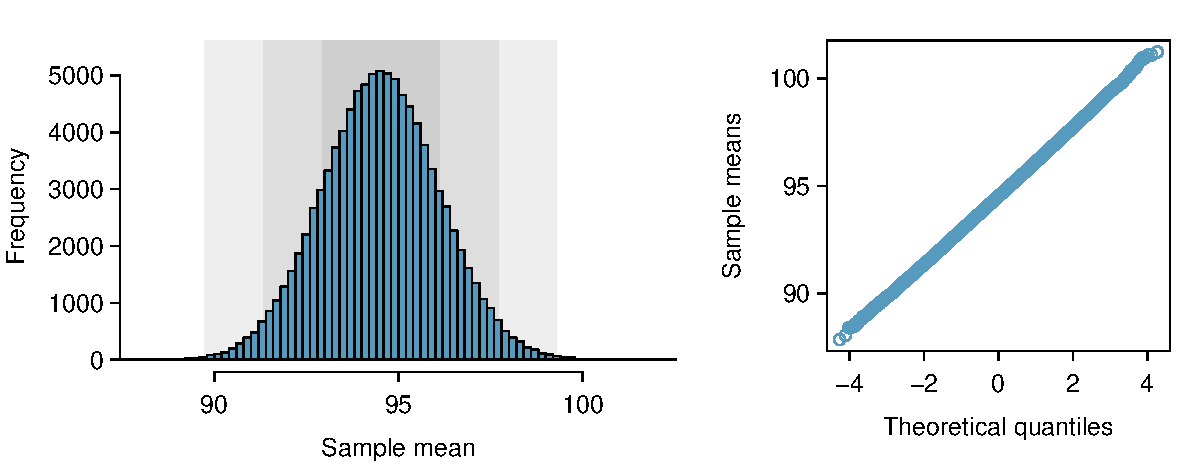
\includegraphics[width=0.9\textwidth]{figures/netTimeBigSamplingDistribution/netTimeBigSamplingDistribution}
	   \caption{The left panel shows a histogram of the sample means for 100,000 different random samples. The right panel shows a normal probability plot of those sample means.}
	\end{figure}
	\[\Downarrow\]
	The distribution of the sample mean is well approximated by a normal model.
\end{frame}
\begin{frame}{Confidence interval}
	\begin{figure}
	\centering
	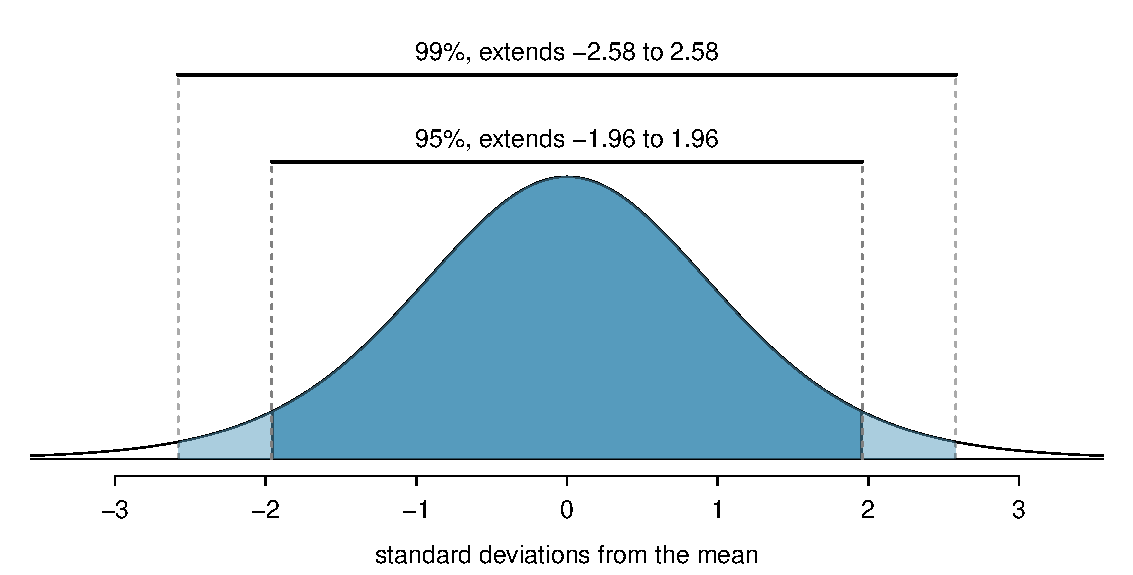
\includegraphics[width=0.7\textwidth]{figures/choosingZForCI/choosingZForCI}\end{figure}
		\begin{itemize}
			\item The 95\% condidence interval for mean estimate is
				\begin{eqnarray*}
				\bar{x}\ \pm\ 1.96\times SE_{\bar{x}}
			\end{eqnarray*}
	\item The 99\% condidence interval for mean estimate is
		\begin{eqnarray*}
		\bar{x}\ \pm\ 2.58\times SE_{\bar{x}}
		\end{eqnarray*}
	\end{itemize}
\end{frame}
\begin{frame}{Checking normality}
	\begin{framed}
		\textbf{Conditions for $\bar{x}$ being nearly normal and $SE$ being accurate}\\
	Important conditions to help ensure the sampling distribution of $\bar{x}$ is nearly normal and the estimate of SE sufficiently accurate:
	\begin{itemize}
	\setlength{\itemsep}{0mm}
	\item The sample observations are independent.
	\item The sample size is large: $n\geq30$ is a good rule of thumb.
	\item The population distribution is not strongly skewed. (We check this using the sample distribution as an estimate of the population distribution.)
	\end{itemize}
	Additionally, the larger the sample size, the more lenient we can be with the sample's skew.
\end{framed}
\end{frame}
\begin{frame}{Checking normality}
	\textbf{Alternative conditions for normality}\\
	If the population of cases is known to be nearly normal and the population standard deviation $\sigma$ is known, then the sample mean $\bar{x}$ will follow a nearly normal distribution $N(\mu, \sigma/\sqrt{n})$ if the sampled observations are also independent.
\end{frame}
\begin{frame}{Confidence interval}
	\begin{framed}
\textbf{Confidence interval for any confidence level}\\
If the point estimate follows the normal model with standard error $SE$, then a confidence interval for the population parameter is
\begin{eqnarray*}
\text{point estimate}\ \pm\ z^{\star} SE
\end{eqnarray*}
where $z^{\star}$ corresponds to the confidence level selected and the standard error is

\[SE=\left\lbrace\begin{array}{lc}
\frac{\sigma}{\sqrt{n}},& \text{if $\sigma$ is known}\\
\frac{s}{\sqrt{n}},& \text{otherwise.}

\end{array}\right.\]

\end{framed}
\end{frame}
\begin{frame}{Confidence interval}
	\textbf{Q:} What does 95\% confident mean?
	If we take a number of samples and construct their confidence intervals, about 95\% will include the actual mean $\mu.$
	\begin{figure}[hht]
	   \centering
	  \caption{Twenty-five samples of size $n=100$ from the run10 data set and their respective confidence intervals.} 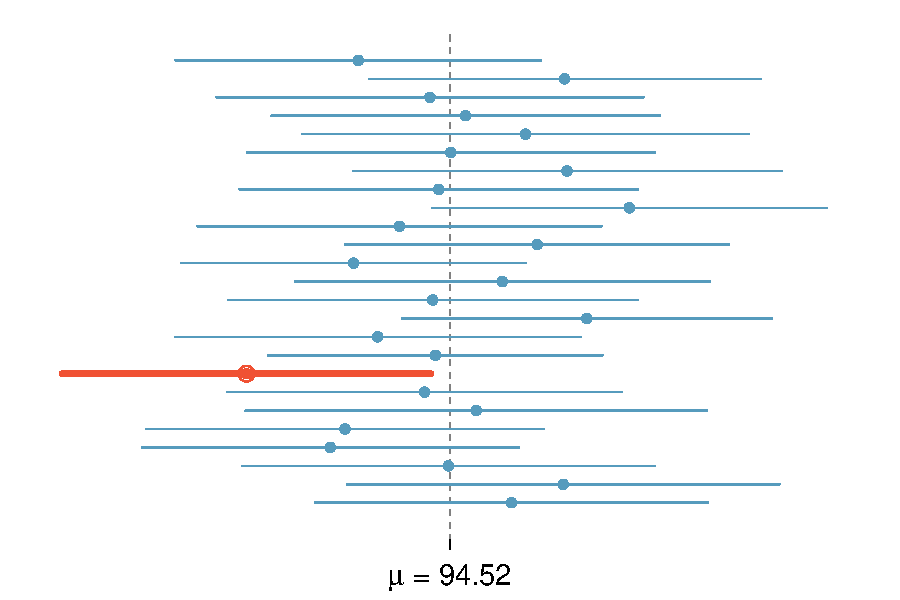
\includegraphics[width=0.7\textwidth]{figures/95PercentConfidenceInterval/95PercentConfidenceInterval}
	\end{figure}
\end{frame}
\begin{frame}{Interpretation}
	
\textbf{Correct interpretation:}\\
We are XX\% confident that the population parameter is between...
\\
\textbf{Example:}
The 95\% confidence interval for the time mean, base on run10Samp, is 

\[(92.45, 98.77)\]

Hence, we are 95\% confident that the population mean in between $92.45$ and  $98.77$.


\end{frame}
\begin{frame}{Hypothesis testing}
	\textbf{Cherry Blossom Run}\\
\begin{itemize}
	\item The average time for all runners who finished the Cherry Blossom Run in 2006 was 93.29.
	\item The sample average time of the sample runners who finished the Cherry Blossom Run in 2012 was 95.61.
	\item Does the sample data from 2012 provides strong evidence that the runners were faster or slower than those in runners in 2006?
\end{itemize}
\end{frame}
\begin{frame}{Hypothesis testing}
	
	\begin{itemize}
	\setlength{\itemsep}{0mm}
	\item[$H_0$:] The average 10 mile run time was the same for 2006 and 2012.
	\item[$H_A$:] The average 10 mile run time for 2012 was \emph{different} than that of 2006.
	\end{itemize}
	We call $H_0$ the \textbf{null hypothesis} and $H_A$ the \textbf{alternative hypothesis}.
\end{frame}
\begin{frame}{Hypothesis testing}
\textbf{Mathematical notation}\vspace{0.3cm}

Let $\mu_{12}$ denote the average run time for 2012. Then the two hypothesis are:
\begin{itemize}
\item[$H_0$:] $\mu_{12} = 93.29$
\item[$H_A$:]$\mu_{12} \neq 93.29$
\end{itemize} 

where $93.29$ minutes is the average 10 mile time for all runners in the 2006 Cherry Blossom Run.
\end{frame}
\begin{frame}{Testing hypotheses using confidence interval}
	\textbf{Cherry Blossom Run}
	\begin{itemize}
		\item Null hypothesis $\mu_{12}=93.29$
		\item Sample mean $\bar{x}_{12}=95.61$
		\item The difference between the $\bar{x}_{12}$ and $93.29$ could be due to \textbf{sampling variation}
	\item  So we turn our attention to the 95\% confidence interval for the time average is
	\[(92.45,98.77)\]
\end{itemize}
\textbf{Conclusion:} Since $93.29$ is in the 95\% confidence interval, we can not reject the null hypothesis. We have not found strong evidence that the average running time in 2012 is different from $93.29$.
\end{frame}
\begin{frame}{Testing hypotheses using confidence interval}
	\begin{itemize}
	\setlength{\itemsep}{0mm}
	\item The null value (the parameter value under the null hypothesis) is in the 95\% confidence interval but just barely, so we would not reject $H_0$. However, we might like to somehow say, quantitatively, that it was a close decision.
	\item The null value is very far outside of the interval, so we reject $H_0$. However, we want to communicate that, not only did we reject the null hypothesis, but it wasn't even close.
	\end{itemize}
\end{frame}

\begin{frame}{Significance level- p-value}
	\textbf{Heuristics}\\
	\begin{itemize}
		\item We do not reject $H_0$ unless we have strong evidence.
		\item What precisely does \emph{strong evidence} mean? 
		 \begin{itemize}
			\item As a general rule of thumb, for those cases where the null hypothesis is actually true, we do not want to incorrectly reject $H_0$ more than $\alpha\%$ of the time.
			\item $\alpha$ is called the significance level.
		\end{itemize}
	\end{itemize}
	\textbf{p-value}
	\begin{figure}[hht]
	\centering
	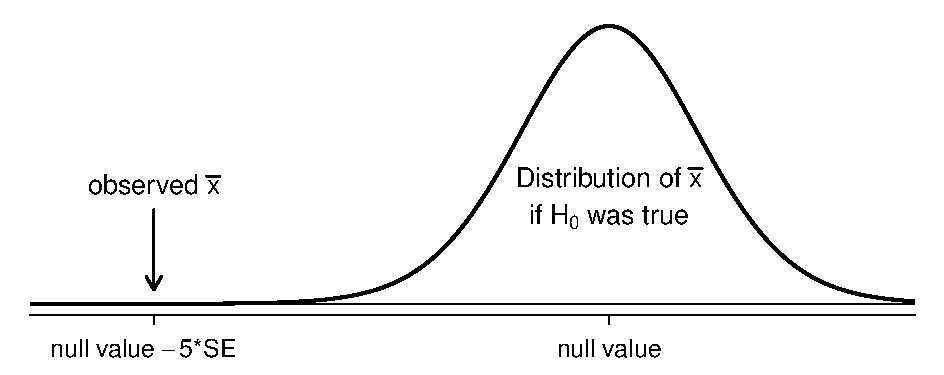
\includegraphics[width=0.75\textwidth]{figures/whyWeWantPValue/whyWeWantPValue}
	\label{whyWeWantPValue}
	\end{figure}
\end{frame}
\begin{frame}{Hypothesis testing- p-values}
	\textbf{Q} How long do students sleep?
	\begin{figure}
	\centering
	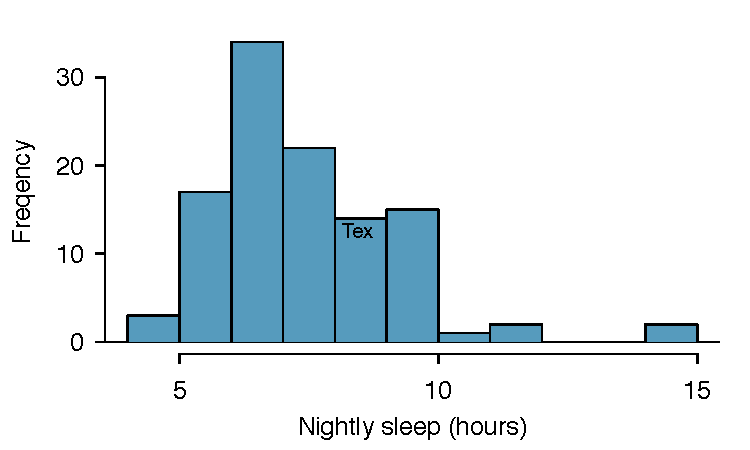
\includegraphics[height=55mm]{figures/histOfSleepForCollegeThatWasCheckingForMoreThan7Hours/histOfSleepForCollegeThatWasCheckingForMoreThan7Hours}
	\caption{Distribution of a night of sleep for 110 college students. }
	\end{figure}
	
\end{frame}
\begin{frame}{Hypothesis testing- p-values}
	\begin{itemize}
		\item A poll by the National Sleep Foundation found that college students average about 7 hours of sleep per night.
		\item The average sleep time in the sample is $\bar{x}=7.42$ hours.
		\item How can we check is the students average more than $7$ hours of sleep?
	\end{itemize}
\end{frame}
\begin{frame}
	\textbf{Hypothesis testing}
	\begin{itemize}
	\setlength{\itemsep}{0mm}
	\item[$H_0$:] $\mu = 7$.
	\item[$H_A$:]$\mu>7$.
\end{itemize}
Evaluate the $Z-$score
\begin{eqnarray*}
Z &=& \frac{\bar{x} - \text{null value}}{SE_{\bar{x}}} = \frac{7.42 - 7}{0.17} = 2.47
\end{eqnarray*}
\[\text{p-value}=P(Z>2.47)=0.07\]
\begin{figure}[hht]
   \centering
   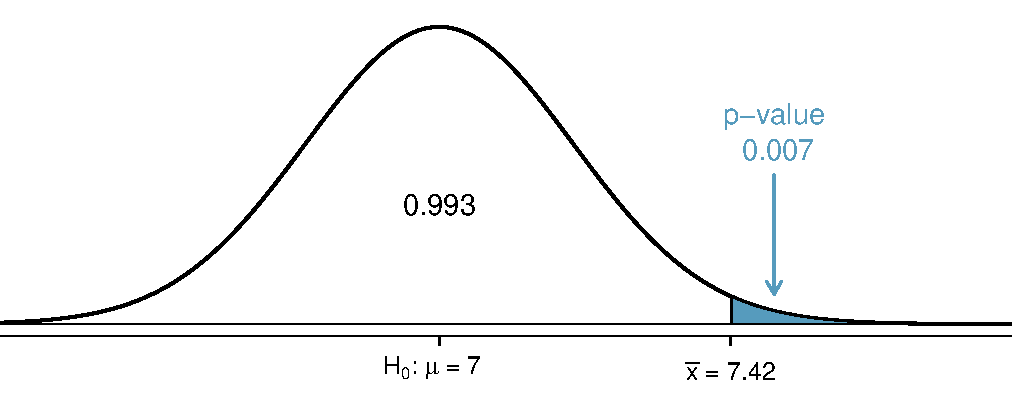
\includegraphics[width=0.73\textwidth]{figures/pValueOneSidedSleepStudy/pValueOneSidedSleepStudy}
  
   \label{pValueOneSidedSleepStudy}
\end{figure}
\end{frame}
\begin{frame}{Hypothesis testing- p-value}
\begin{itemize}
	\item If the null hypothesis is true, the probability of observing such a large sample mean for a sample of 110 students is only 0.007.
	\item We evaluate the hypotheses by comparing the p-value to the significance level.
	\item Since $p-value=0.007<0.05=\alpha$ we reject the null hypothesis.
\end{itemize}
\begin{framed}
The p-value quantifies how strongly the data favour $H_A$ over $H_0$. A small p-value (usually $<0.05$) corresponds to sufficient evidence to reject $H_0$ in favour of $H_A$.
\end{framed}
\end{frame}
\begin{frame}{Hypothesis testing - p-value}
	\textbf{$\alpha-$ level Hypothesis Testing}
		\begin{itemize}
		\setlength{\itemsep}{0mm}
		\item[$H_0$:] $\mu = \mu_0$.
		\item[$H_A$:]$\left\{
		\begin{array}{ll}
			\mu>\mu_0& \text{(upper-tail alternative)}\\
			\mu\neq\mu_0& \text{(two-tailed alternative)}\\
			\mu< \mu_0& \text{(lower-tail alternative)}
		\end{array}
		\right.$
	\end{itemize}
	Test statistic: $Z=\frac{\hat{x}-\mu_0}{SE}$\\
	We reject $H_0$ when:
	\begin{itemize}
		\item $P(Z>z)<\alpha$ (upper-tail alternative)
		\item $P(|Z|>z)<\alpha$ (two-tailed alternative)
		\item $P(Z<-z)<\alpha$ (lower-tail alternative)
\end{itemize}
\end{frame}
\begin{frame}{Decision errors}
	
	\begin{table}[ht]
	\centering
	\resizebox{0.8\textwidth}{!}{
	\begin{tabular}{l l c c}
	& & \multicolumn{2}{c}{\textbf{Test conclusion}} \\
	  \cline{3-4}
	\vspace{-3.7mm} \\
	& & do not reject $H_0$ &  reject $H_0$ in favor of $H_A$ \\
	  \cline{2-4}
	\vspace{-3.7mm} \\
	& $H_0$ true & okay &  Type~1 Error \\
	\raisebox{1.5ex}{\textbf{Truth}} & $H_A$ true & Type 2 Error & okay \\
	  \cline{2-4}
	\end{tabular}}
		\end{table}
		\small\begin{itemize}
			\item\textbf{Type 1 Error} is rejecting the null hypothesis when $H_0$ is actually true. 
			\item\textbf{Type 2 Error} is failing to reject the null hypothesis when the alternative is actually true.
		\end{itemize}
\end{frame}
\end{document}